\documentclass[11pt]{beamer}
\usetheme{Frankfurt}
\usecolortheme{default}
\usefonttheme{professionalfonts}

\usepackage[utf8x]{inputenc}
%\usepackage[T1]{fontenc}


% update font maps?
\usepackage{sansmathaccent}
\pdfmapfile{+sansmathaccent.map}
% Block diagram packages
\usepackage{tikz}
\usetikzlibrary{shapes,arrows}
\usepackage{verbatim}

% Arrow 
\usetikzlibrary{decorations.markings}
\usepackage{amsmath}% align equal signs
\tikzstyle{block} = [draw, fill=white, rectangle, 
    minimum height=3em, minimum width=6em]
\tikzstyle{sum} = [draw, fill=white, circle, node distance=1cm]
\tikzstyle{input} = [coordinate]
\tikzstyle{output} = [coordinate]
\tikzstyle{pinstyle} = [pin edge={to-,thin,black}]
\def\doubleunderline#1{\underline{\underline{#1}}}

\graphicspath{{/home/rajiv/IIB/year4project/report/figures/}}
\DeclareGraphicsExtensions{.png,.jpg,.PNG,.jpeg}

\begin{document}
\author{Rajiv Kurien}
\title{Relay feedback models of biological oscillators}
%\subtitle{Karl J. \r{A}str\"{o}m  (1995)}
%logo{}
%\institute[CUED]{Cambridge University Engineering Department}
\date{ 1 June 2016}
%\subject{IIB Project }
\setbeamercovered{transparent}
\setbeamertemplate{navigation symbols}{}

\begin{frame}
\titlepage
% The block diagram code is probably more verbose than necessary

\end{frame}


\section{Introduction}

\subsection{Relay feedback}
\subsubsection{Relay}

\begin{frame}
\frametitle{Relay}
  \tikzstyle arrowstyle=[scale=2]
  \tikzstyle directed=[postaction={decorate,decoration={markings,
      mark=at position .9 with {\arrow[arrowstyle]{stealth}}}, mark = at position .9 with {\arrow[arrowstyle]{stealth}}}]
  \begin{center}
  \begin{tikzpicture}[scale = 1]
    \draw [->, very thick] (-3,0)  node (xaxis_right){} -- (3, 0) node (xaxis_left) [below] {\LARGE  $e$};
    \draw [->, very thick] (0,-3)  node (yaxis_bottom){} -- (0, 3) node (yaxis_top) [right] {\LARGE $u$};
    \draw [directed, thick, blue] (3,2) node(relay_top_right){} --(-1,2) node (relay_top_left){};
    \draw[directed, thick, blue] (-3,-2) node(relay_bottom_left){}--(1,-2) node (relay_bottom_right){};
    \draw[directed, thick, blue] (-1,2) node{} -- (-1,-2) node {};
    \draw[directed, thick, blue] (1,-2) node{} -- (1,2) node {};

    \draw (1,0) node [below right]{\LARGE $\epsilon$}; %label
    \draw (-1,0) node [below left]{\LARGE $-\epsilon$}; %label
    \draw (0,2) node [above left]{\LARGE $d$}; %label
    \draw (0,-2) node [below left]{\LARGE $-d$}; %label
	\end{tikzpicture}
	\end{center}
\end{frame}

\subsubsection{Relay feedback}
\begin{frame}
\frametitle{Relay feedback}

\tikzstyle{block} = [draw, fill=white, rectangle, 
    minimum height=3em, minimum width=6em,text width = 1cm, align = center]
\tikzstyle{sum} = [draw, fill=white, circle, node distance=1cm]
\tikzstyle{input} = [coordinate]
\tikzstyle{output} = [coordinate]
\tikzstyle{pinstyle} = [pin edge={to-,thin,black}]

% The block diagram code is probably more verbose than necessary
\begin{center}
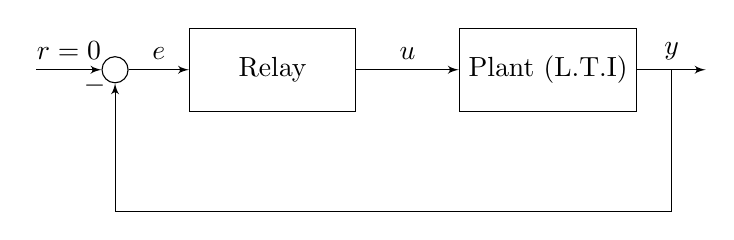
\begin{tikzpicture}[auto, node distance=2cm,>=latex']
    % We start by placing the blocks
    \node [input, name=input] {};
    \node [sum, right of=input] (sum) {};
    \node [block, right of=sum] (relay) {Relay};
    \node [block, right of=relay, node distance = 3.5cm] (plant) {Plant (L.T.I)};
    % We draw an edge between the controller and system block to 
    % calculate the coordinate u. We need it to place the measurement block. 
    \draw [->] (relay) -- node[name=u] {$u$} (plant);
    \node [output, right of=plant] (output) {};
    \node [output, below of=u] (measurements) {Measurements};

    % Once the nodes are placed, connecting them is easy. 
    \draw [draw,->] (input) -- node {$r = 0$} (sum);
    \draw [->] (sum) -- node {$e$} (relay);
    \draw [->] (plant) -- node [name=y] {$y$}(output);
    \draw [-] (y) |- (measurements);
    \draw [->] (measurements) -| node[pos=0.99] {$-$} 
        node [near end] {} (sum);
\end{tikzpicture}
\end{center}

\begin{figure}
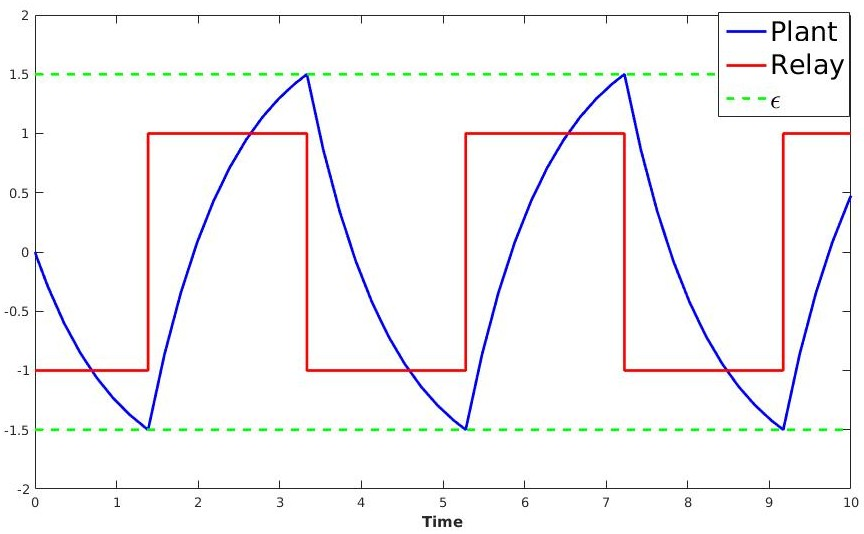
\includegraphics[width = 0.65\textwidth]{relay_feedback}
\end{figure}

\end{frame}

\begin{frame}
\frametitle{Oscillations in relay feedback systems}
\framesubtitle{\r{A}str\"{o}m. \emph{Oscillations in systems with relay feedback.} (1995)}
Analytical solutions for:
\begin{itemize}
\item Time period of oscillations
\item Stability of oscillations
\item Initial conditions for oscillations
\end{itemize}
\begin{figure}
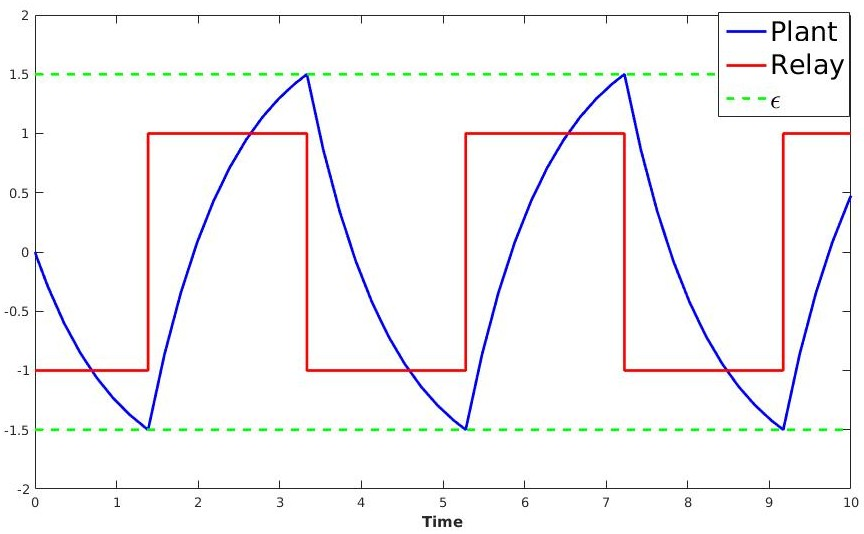
\includegraphics[width = 0.65\textwidth]{relay_feedback}
\end{figure}
\end{frame}

%\subsection{Motivation}
%\begin{frame}
%\frametitle{Motivation}
%\begin{itemize}
%\item Auto-tuning of process controllers
%\item Model biological oscillations
%\end{itemize}
%\end{frame}

\begin{frame}%[shrink=30]
\frametitle{Models of biological oscillations}
\framesubtitle{Goldbeter. \emph{A model for circadian oscillations in the Drosophila period protein}. (1995) }

\begin{figure}
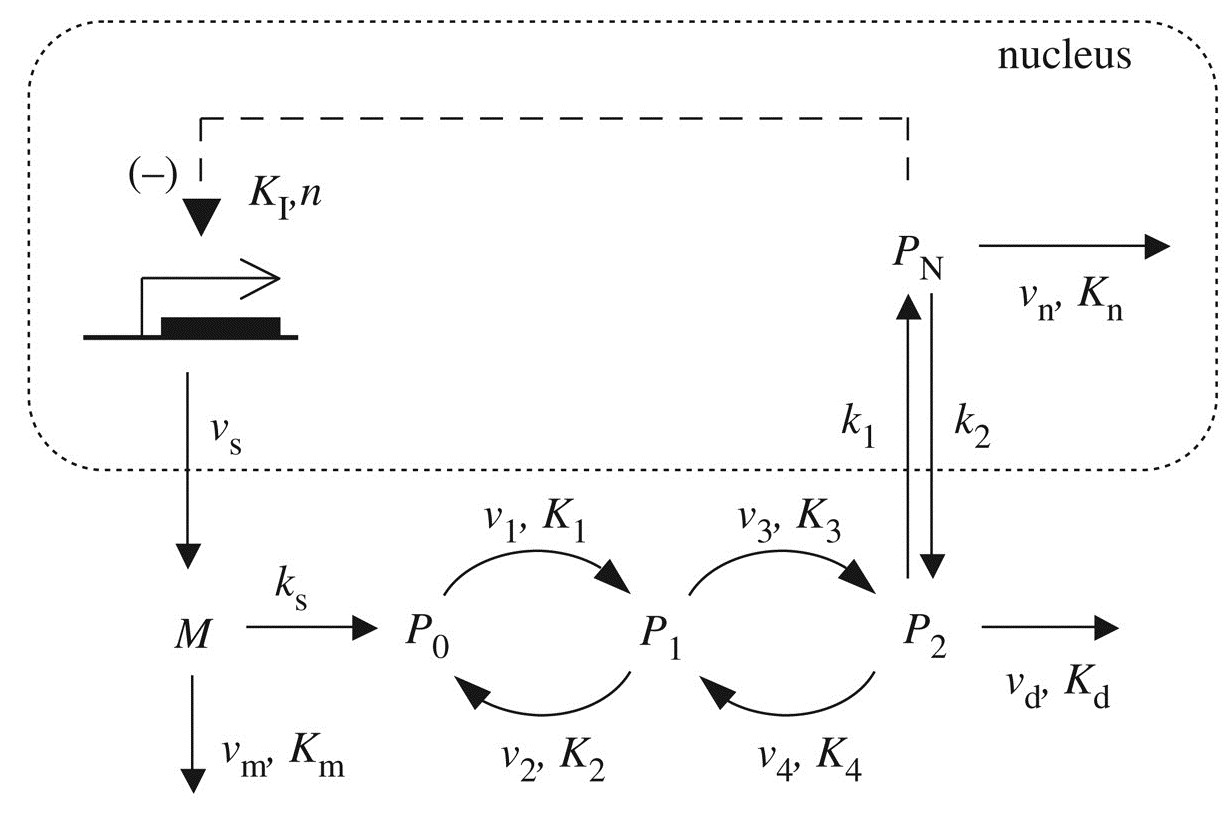
\includegraphics[width = 0.5\textwidth]{goldbeter_model}
\end{figure}

%\column{.6\textwidth}
\begin{center}
\tiny
\begin{align*}
%
\frac{dM}{dt}   &= v_s\frac{K_I^n}{K_I^n + P_N^n} - v_m\frac{M}{K_m + M} \\
\frac{dP_0}{dt} &= k_sM - v_1\frac{P_0}{K_1 + P_0} + v_2\frac{P_1}{K_2 + P_1} \\
\frac{dP_1}{dt} &= v_1\frac{P_0}{K_1 + P_0} - v_2\frac{P_1}{K_2 + P_1} - v_3\frac{P_1}{K_3 + P_1} + v_4\frac{P_2}{K_4 + P_2} \\
\frac{dP_2}{dt} &= v_3\frac{P_1}{K_3 + P_1} - v_4\frac{P_2}{K_4 + P_2} - v_d\frac{P_2}{K_d + P_2} - k_1P_2 + k_2P_N\\
\frac{dP_N}{dt} &= k_1P_2 - k_2P_N -v_n\frac{P_N}{K_n + P_N}\\
%
%
\end{align*}

\end{center}

\end{frame}

\begin{frame}
\frametitle{Models of biological oscillations}
\begin{itemize}
\item Difficult to analyse oscillations
\item Tuning of parameters
\item Relay feedback framework
\end{itemize}

Are relay feedback models appropriate to analyse biological oscillations?
\end{frame}

\subsection{Outline}
\begin{frame}
	\frametitle{Project outline}
Are relay feedback models appropriate to analyse biological oscillations?	
\begin{itemize}
\item Simple oscillations
\begin{itemize}
\item Goodwin Oscillator model for circadian rhythms
\item FitzHugh-Nagumo model for action potentials
\end{itemize}
\item Complex oscillations
\begin{itemize}
\item Bursting normal form
\item Hindmarsh-Rose model for bursting
\end{itemize}
\end{itemize}
\end{frame}

\begin{comment}
\section{Goodwin Oscillator}
\subsection{Intro}
\begin{frame}
	\frametitle{Goodwin Oscillator}
	
	\begin{itemize}
	\item Biochemical oscillator based on negative feedback
	\item Concentration of mRNA, protein and end product
	\end{itemize}
	
\begin{columns}
\column{0.8\textwidth}
	\begin{align*}
	\text{mRNA \hspace{1cm}}\frac{dx_1}{dt'} &= \frac{1}{1 + x_3^p} - b_1x_1 \\
	\text{Protein \hspace{1cm}}	\frac{dx_2}{dt'} &= b_2(x_1 - x_2) \\
	\text{Product \hspace{1cm}}	\frac{dx_3}{dt'} &= b_3(x_2 - x_3) \\
	\end{align*}
\column{0.2\textwidth}
\end{columns}
%	\begin{figure}
%	\includegraphics<2>\\[width=0.7\textwidth]{goodwin_nonlinear_element}
%	\end{figure}

\end{frame}

\begin{frame}
\frametitle{Goodwin Oscillator}
\begin{figure}
	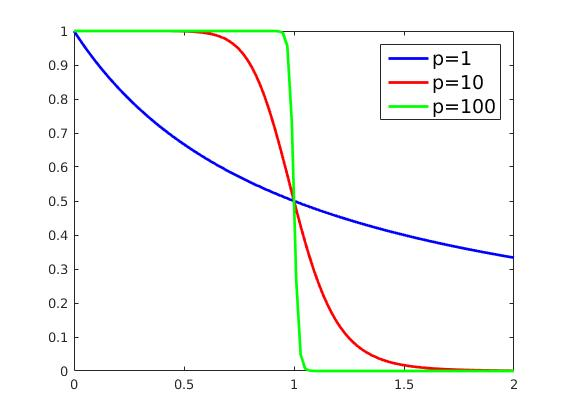
\includegraphics[width=0.7\textwidth]{goodwin_nonlinearity}
\end{figure}
\end{frame}

\subsection{Timescale}
\begin{frame}
	\frametitle{Separation of timescales}
	
	\begin{itemize}
	\item Fast positive feedback
	\item Slow negative feedback
	\end{itemize}
	
\begin{columns}
\column{0.8\textwidth}
	\begin{align*}
	\text{mRNA \hspace{1cm}}\frac{dx_1}{dt'} &= \frac{1}{1 + x_3^p} - b_1x_1 \\
	\text{Protein \hspace{1cm}}	\frac{dx_2}{dt'} &= b_2(x_1 - x_2) \\
	\text{Product \hspace{1cm}}	\frac{dx_3}{dt'} &= b_3(x_2 - x_3) \\
	\end{align*}
\column{0.2\textwidth}
\begin{figure}
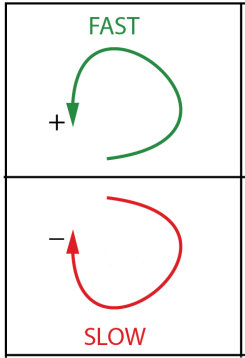
\includegraphics[width=\textwidth]{feedback}
\end{figure}
\end{columns}
%	\begin{figure}
%	\includegraphics<2>\\[width=0.7\textwidth]{goodwin_nonlinear_element}
%	\end{figure}

\end{frame}

\subsection{Modelling with relay feedback}
\begin{frame}
\frametitle{Goodwin Oscillator and Relay Feedback}
\begin{columns}
\column{0.5\textwidth}
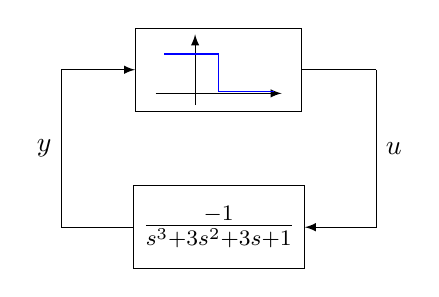
\begin{tikzpicture}[auto, node distance=2cm,>=latex]
\tikzstyle{block} = [draw,  rectangle,  minimum height=3em, minimum width=6em]
\tikzstyle{sum} = [draw,  circle, node distance=1cm]
\tikzstyle{input} = [coordinate]
\tikzstyle{output} = [coordinate]
\tikzstyle{pinstyle} = [pin edge={to-,thin,black}]   % We start by placing the blocks

\def\relay{
\tikz[remember picture,overlay]{
\draw[->] (-.8,-.3) -- (.8,-0.3);
\draw[->] (-.3,-0.45)--(-.30,0.45);
\draw[blue] (0.7,-0.28)--(0.,-0.28)--(0,0.2)--(-.7,.2);
%\draw[blue] (-.2,.2)--(-.2,-.2)--(.2,-.2);
}}

    \node [block] (inverse) {};
    \node[] at (inverse) {\relay};
    \node [output, right of = inverse] (output) {};
    \node [input, left of = inverse](input){};
    \node [block, below of = inverse](linear_tf){\large $\frac{-1}{s^3 + 3s^2 + 3s + 1}$};

    % Once the nodes are placed, connecting them is easy. 
    \draw [-] (inverse) -- (output);
    \draw [->] (output) |- node[near start] {$u$}(linear_tf);
    \draw [-] (linear_tf) -| node[near end] {$y$} (input);
    \draw [->] (input) -- (inverse);

\end{tikzpicture}
\column{0.5\textwidth}
\begin{figure}
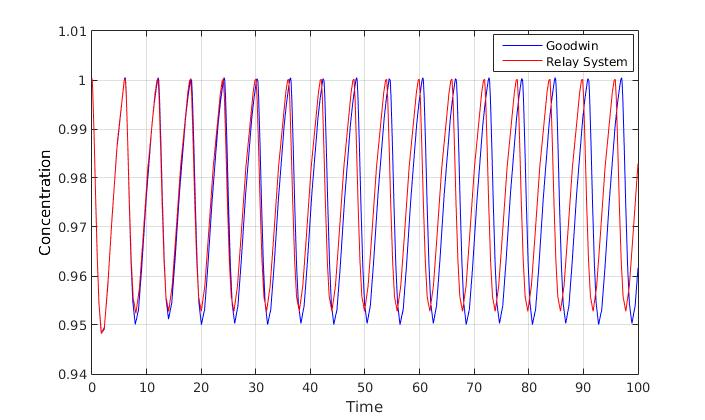
\includegraphics[width=\textwidth]{goodwin_mathcing}
\end{figure}
\end{columns}
\end{frame}

\end{comment}
\section{FitzHugh-Nagumo}

\subsection{Introduction}

\begin{frame}
\frametitle{FitzHugh-Nagumo (1961)}

\begin{itemize}
\item Action potential in a neuron
\item Hodgkin-Huxley simplified to two variables
\item Excitable system
\end{itemize}
\begin{columns}
\column{0.5\textwidth}
\begin{figure}
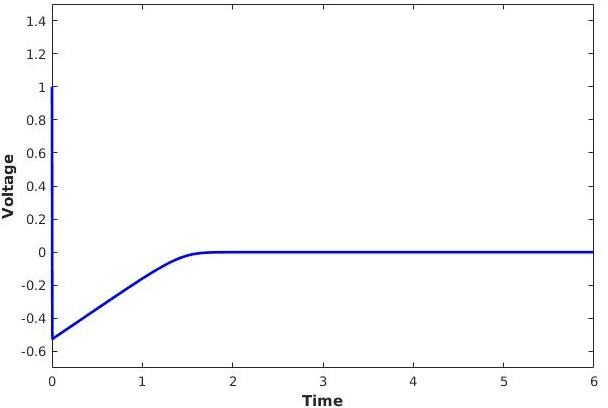
\includegraphics[width = \textwidth]{fn2}
\end{figure}
\column{0.5\textwidth}
\begin{figure}
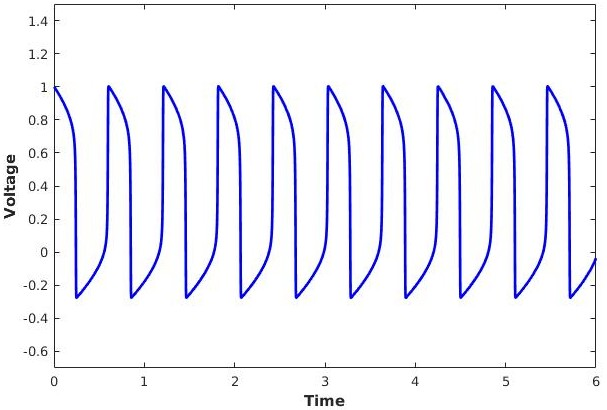
\includegraphics[width = \textwidth]{fn1}
\end{figure}
\end{columns}
\end{frame}

\begin{frame}
\frametitle{FitzHugh-Nagumo (1961)}
\begin{columns}
\column{0.5\textwidth}
	\begin{align*}
	\text{Voltage\hspace{0.5cm} }\epsilon\frac{dv}{dt} &= f(v) - i + I_{\text{app}} \\
	\text{Current\hspace{0.7cm} }\frac{di}{dt} &= v - \gamma i\\
	\end{align*}
	\column{0.5\textwidth}
\centering
\tikzstyle{block} = [draw,  rectangle,  minimum height=3em, minimum width=6em]
\tikzstyle{sum} = [draw,  circle, node distance=1cm]
\tikzstyle{input} = [coordinate]
\tikzstyle{output} = [coordinate]
\tikzstyle{pinstyle} = [pin edge={to-,thin,black}]
\resizebox{5cm}{!}{%
  % The block diagram code is probably more verbose than necessary
  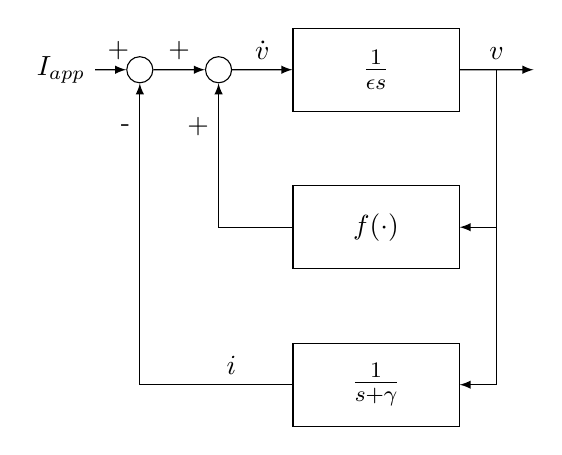
\begin{tikzpicture}[auto, node distance=2cm,>=latex,scale=0.75]
      % We start by placing the blocks
      \node at (0,3) (I_app) {$I_{app}$};
      %\node[input, name = I_app]{text};
      \node[sum, right of = I_app](sum_outer){};
      \node [sum, right of = sum_outer] (sum_inner) {};
      \node [block, right of = sum_outer, node distance=3cm] (high_gain) {\large{$\frac{1}{\epsilon s}$}};
      % We draw an edge between the controller and system block to 
      % calculate the coordinate u. We need it to place the measurement block. 
      \node [output, right of = high_gain] (output) {};
      \node [block, below of = high_gain] (cubic_nullcline) {$f(\cdot)$};
      \node [block, below of = cubic_nullcline](linear_tf){\large $\frac{1}{s+\gamma}$};

      % Once the nodes are placed, connecting them is easy. 

      % inner loop
      \draw [draw,->] (sum_outer) -- node {$+$} (sum_inner);
      \draw [->] (sum_inner) -- node {$\dot{v}$} (high_gain);
      \draw [->] (high_gain) -- node [name=v] {$v$}(output);
      \draw [->] (v) |- (cubic_nullcline);
      \draw [->] (cubic_nullcline) -| node[pos=.85] {$+$} 
          node [near end] {} (sum_inner);

      % outer loop
      \draw [->](v) |- (linear_tf);
      \draw [->](linear_tf) -| node[anchor=south,pos=0.2] {$i$} 
          node[pos=0.93]{-}(sum_outer);
      \draw [->](I_app)-- node[near end]{$+$} (sum_outer);
  \end{tikzpicture}}
	\end{columns}

\end{frame}

\subsection{Typical oscillations}
\begin{frame}
\frametitle{FitzHugh-Nagumo}

	\begin{columns}
		\column{.5\textwidth}
		\begin{figure}
		        %\includegraphics<1>[width=\textwidth]{tmr_fn_limit_cycle}
		        \includegraphics<1>[width=\textwidth]{fn_phase_portrait}


		\end{figure}
		
		\column{.5\textwidth}
		\begin{figure}
		       % \includegraphics<1>[width=\textwidth]{tmr_fn_voltage}
				\includegraphics<1>[width=\textwidth]{fn_voltage_time}

		\end{figure}
	\end{columns}
\end{frame}

\begin{comment}
\begin{frame}
\frametitle{Cubic nonlinearity}
\begin{figure}
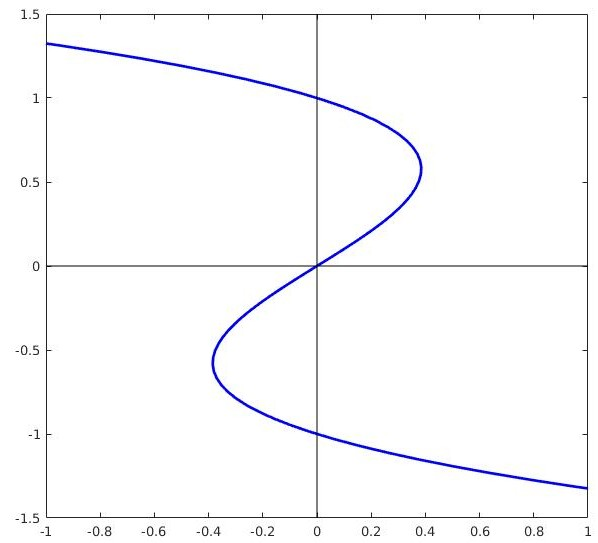
\includegraphics[width = 0.5\textwidth]{cubic.jpg}
\end{figure}
\end{frame}
\end{comment}

\subsection{Feedback}
\begin{frame}
\frametitle{Positive feedback}
\begin{columns}
\column{0.7\textwidth}
\centering
\tikzstyle{block} = [draw,  rectangle,  minimum height=3em, minimum width=6em]
\tikzstyle{block2} = [draw,  rectangle,  minimum height=4em, minimum width=7em]
\tikzstyle{gain} = [draw, regular polygon, regular polygon sides = 3, regular polygon rotate = 90, minimum height = 2em, minimum width = 2em]
\tikzstyle{gain2} = [draw, regular polygon, regular polygon sides = 3, regular polygon rotate = 30, minimum height = 2em, minimum width = 2em]
\tikzstyle{sum} = [draw,  circle, node distance=1cm]
%\tikzstyle{input} = [coordinate]
%\tikzstyle{output} = [coordinate]
\tikzstyle{pinstyle} = [pin edge={to-,thin,black}]

\def\saturationA
{
	\tikz[remember picture,overlay]
	{
		\draw[->] (-.5,0) -- (.5,0);
		\draw[->] (0,-.5)--(0,.5);
		\draw[blue] (-.5,-.3)--(-.1,-.3)--(.1,.3)--(.5,.3);
		\node at (-.2,0.1) {\tiny$-1$};
		\node at (.1,-0.1) {\tiny$1$};
	}
}

\def\saturationB
{
	\tikz[remember picture,overlay]
	{
		\draw[->] (-1,0) -- (1,0);
		\draw[->] (0,-.75)--(0,.75);
		\draw[blue] (-1,-.5)--(.3,-.5)--(-.3,.5)--(1,.5);
		\node at (-.45,0.1) {\tiny$1-\beta$};
		\node at (.45,-0.15) {\tiny$\beta-1$};
	}
}

\resizebox{8cm}{!}{%
  % The block diagram code is probably more verbose than necessary
  \begin{tikzpicture}[auto, node distance=2cm,>=latex,scale=.25]
      % We start by placing the blocks
      
      % Orignal loop
      \node [block]at (0,-3) (satA){};
      \node [] at (satA) {\saturationA};
      \node [coordinate, right of = satA](endB){};
      \node [gain, above of = satA](beta){ $\beta$};
      \node [left of = beta](inB){};
      

      % Once the nodes are placed, connecting them is easy. %

	% ultra-slow loop
	\draw[-](satA)--(endB);
	\draw[->](endB)|- node[name = middlepoint, near start]{} (beta); 
	\draw[-](beta)--(inB);
	\draw[->](inB)|-node[pos=.5, name = edgejoint]{} (satA);
	\draw[-](beta)-|(edgejoint);
     
     % Equal to sign
     \node[right of = middlepoint, node distance = .7cm](equalToSign){\large $=$};
     \node [block2, right of = equalToSign, node distance = 2cm](saturationB){};
     \node [] at (saturationB) {\saturationB};     

  \end{tikzpicture}
}
\column{0.3\textwidth}
\begin{figure}
%\includegraphics[width=0.8\textwidth]<1>{positive}
\end{figure}
\end{columns}
\end{frame}

\begin{frame}
\frametitle{Positive feedback}
\begin{columns}
\column{0.7\textwidth}
\centering
\tikzstyle{block} = [draw,  rectangle,  minimum height=3em, minimum width=6em]
\tikzstyle{block2} = [draw,  rectangle,  minimum height=4em, minimum width=7em]
\tikzstyle{gain} = [draw, regular polygon, regular polygon sides = 3, regular polygon rotate = 90, minimum height = 2em, minimum width = 2em]
\tikzstyle{gain2} = [draw, regular polygon, regular polygon sides = 3, regular polygon rotate = 30, minimum height = 2em, minimum width = 2em]
\tikzstyle{sum} = [draw,  circle, node distance=1cm]
%\tikzstyle{input} = [coordinate]
%\tikzstyle{output} = [coordinate]
\tikzstyle{pinstyle} = [pin edge={to-,thin,black}]

\def\saturationA
{
	\tikz[remember picture,overlay]
	{
		\draw[->] (-.5,0) -- (.5,0);
		\draw[->] (0,-.5)--(0,.5);
		\draw [blue] plot [smooth] coordinates{ (-.5,-.35)(-.15,-.3)(.15,.3)(.5,.35)};
		\node at (-.2,0.1) {\tiny$-1$};
		\node at (.1,-0.1) {\tiny$1$};
	}
}

\def\saturationB
{
	\tikz[remember picture,overlay]
	{
		\draw[->] (-1,0) -- (1,0);
		\draw[->] (0,-.75)--(0,.75);
		\draw[blue] plot [smooth] coordinates{ (-1,-.55)(.3,-.5)(-.3,.5)(1,.55)};
		%\node at (-.45,0.1) {\tiny$1-\beta$};
		%\node at (.45,-0.15) {\tiny$\beta-1$};
	}
}

\resizebox{8cm}{!}{%
  % The block diagram code is probably more verbose than necessary
  \begin{tikzpicture}[auto, node distance=2cm,>=latex,scale=.25]
      % We start by placing the blocks
      
      % Orignal loop
      \node [block]at (0,-3) (satA){};
      \node [] at (satA) {\saturationA};
      \node [coordinate, right of = satA](endB){};
      \node [gain, above of = satA](beta){ $\beta$};
      \node [left of = beta](inB){};
      

      % Once the nodes are placed, connecting them is easy. %

	% ultra-slow loop
	\draw[-](satA)--(endB);
	\draw[->](endB)|- node[name = middlepoint, near start]{} (beta); 
	\draw[-](beta)--(inB);
	\draw[->](inB)|-node[pos=.5, name = edgejoint]{} (satA);
	\draw[-](beta)-|(edgejoint);
     
     % Equal to sign
     \node[right of = middlepoint, node distance = .7cm](equalToSign){\large $=$};
     \node [block2, right of = equalToSign, node distance = 2cm](saturationB){};
     \node [] at (saturationB) {\saturationB};     

  \end{tikzpicture}
}
\column{0.3\textwidth}
\begin{figure}
\includegraphics[width=0.8\textwidth]<1>{positive}
\end{figure}
\end{columns}
\end{frame}

\begin{frame}
\frametitle{Separation of timescales}
\begin{columns}
\column{0.5\textwidth}
\centering
\tikzstyle{block} = [draw,  rectangle,  minimum height=3em, minimum width=6em]
\tikzstyle{sum} = [draw,  circle, node distance=1cm]
\tikzstyle{input} = [coordinate]
\tikzstyle{output} = [coordinate]
\tikzstyle{pinstyle} = [pin edge={to-,thin,black}]
\resizebox{5cm}{!}{%
  % The block diagram code is probably more verbose than necessary
  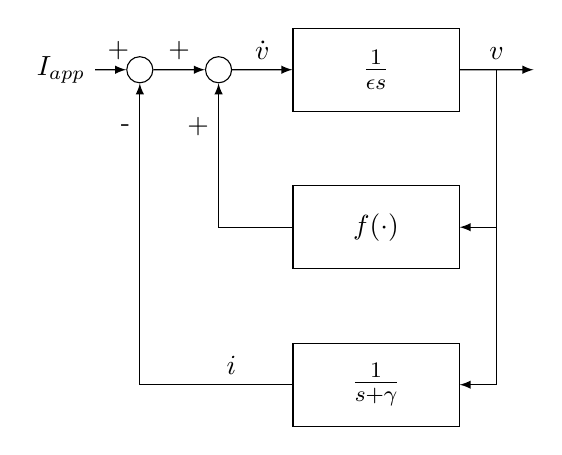
\begin{tikzpicture}[auto, node distance=2cm,>=latex,scale=0.75]
      % We start by placing the blocks
      \node at (0,3) (I_app) {$I_{app}$};
      %\node[input, name = I_app]{text};
      \node[sum, right of = I_app](sum_outer){};
      \node [sum, right of = sum_outer] (sum_inner) {};
      \node [block, right of = sum_outer, node distance=3cm] (high_gain) {\large{$\frac{1}{\epsilon s}$}};
      % We draw an edge between the controller and system block to 
      % calculate the coordinate u. We need it to place the measurement block. 
      \node [output, right of = high_gain] (output) {};
      \node [block, below of = high_gain] (cubic_nullcline) {$f(\cdot)$};
      \node [block, below of = cubic_nullcline](linear_tf){\large $\frac{1}{s+\gamma}$};

      % Once the nodes are placed, connecting them is easy. 

      % inner loop
      \draw [draw,->] (sum_outer) -- node {$+$} (sum_inner);
      \draw [->] (sum_inner) -- node {$\dot{v}$} (high_gain);
      \draw [->] (high_gain) -- node [name=v] {$v$}(output);
      \draw [->] (v) |- (cubic_nullcline);
      \draw [->] (cubic_nullcline) -| node[pos=.85] {$+$} 
          node [near end] {} (sum_inner);

      % outer loop
      \draw [->](v) |- (linear_tf);
      \draw [->](linear_tf) -| node[anchor=south,pos=0.2] {$i$} 
          node[pos=0.93]{-}(sum_outer);
      \draw [->](I_app)-- node[near end]{$+$} (sum_outer);
  \end{tikzpicture}}

\column{0.5\textwidth}
\begin{figure}
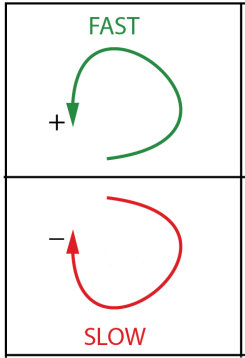
\includegraphics[width = 0.5\textwidth]{feedback}
\end{figure}
\end{columns}
\end{frame}

\subsection{Modelling using relay feedback}
\begin{frame}
\frametitle{FitzHugh-Nagumo and Relay feedback}
\begin{columns}
\column{0.5\textwidth}
\begin{center}
		        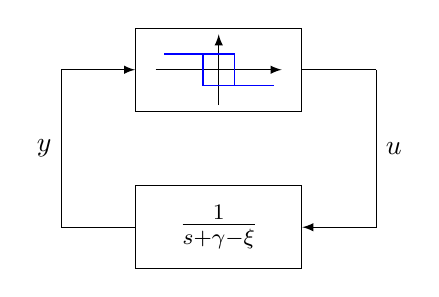
\begin{tikzpicture}[auto, node distance=2cm,>=latex, scale = 0.25]
\tikzstyle{block} = [draw,  rectangle,  minimum height=3em, minimum width=6em]
\tikzstyle{sum} = [draw,  circle, node distance=1cm]
\tikzstyle{input} = [coordinate]
\tikzstyle{output} = [coordinate]
\tikzstyle{pinstyle} = [pin edge={to-,thin,black}]   % We start by placing the blocks

\def\relay{
\tikz[remember picture,overlay]{
\draw[->] (-.8,0) -- (.8,0);
\draw[->] (0,-0.45)--(0,0.45);
\draw[blue] (0.7,-0.2)--(0.2,-0.2)--(0.2,0.2)--(-.7,.2);
\draw[blue] (-.2,.2)--(-.2,-.2)--(.2,-.2);
}}

    \node [block] (inverse) {};
    \node[] at (inverse) {\relay};
    \node [output, right of = inverse] (output) {};
    \node [input, left of = inverse](input){};
    \node [block, below of = inverse](linear_tf){\large $\frac{1}{s+\gamma-\xi}$};

    % Once the nodes are placed, connecting them is easy. 
    \draw [-] (inverse) -- (output);
    \draw [->] (output) |- node[near start] {$u$}(linear_tf);
    \draw [-] (linear_tf) -| node[near end] {$y$} (input);
    \draw [->] (input) -- (inverse);

\end{tikzpicture}
\end{center}
\column{0.5\textwidth}
\begin{figure}
%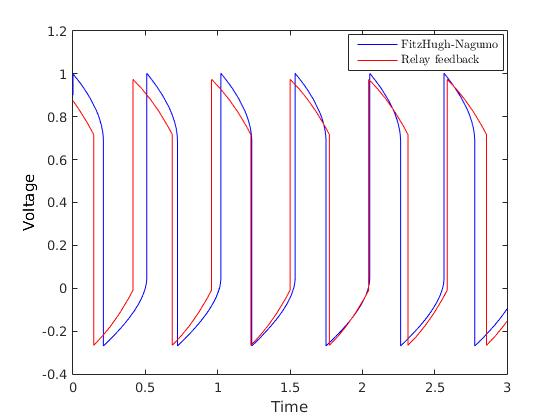
\includegraphics[width = \textwidth]{tmr_fn_relay_voltage}
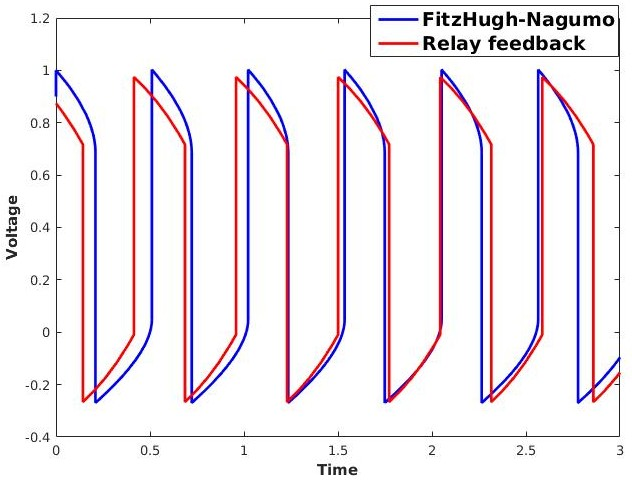
\includegraphics[width = \textwidth]{fn_relay}

\end{figure}
\end{columns}
\end{frame}

\section{Bursting}
\subsection{Introduction}
\begin{frame}
\frametitle{Bursting}
\begin{figure}
\includegraphics[width=.7\textwidth]{typical_bursting}
\end{figure}
\end{frame}

\begin{frame}
\frametitle{Bursting}
\begin{itemize}
\item Important role in signalling mechanisms
\item Neuroendocrine cells and nerve cells
\item Very few tools to analyse bursting
\end{itemize}
\begin{columns}
\column{0.5\textwidth}
\begin{figure}
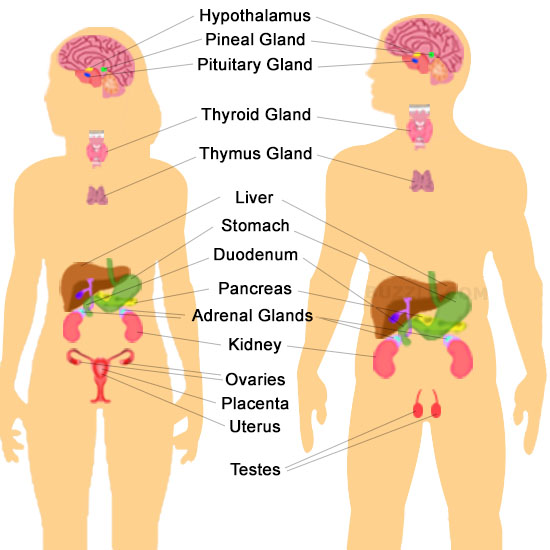
\includegraphics[width=\textwidth]{endocrine-glands}
\end{figure}
\column{0.5\textwidth}
\begin{figure}
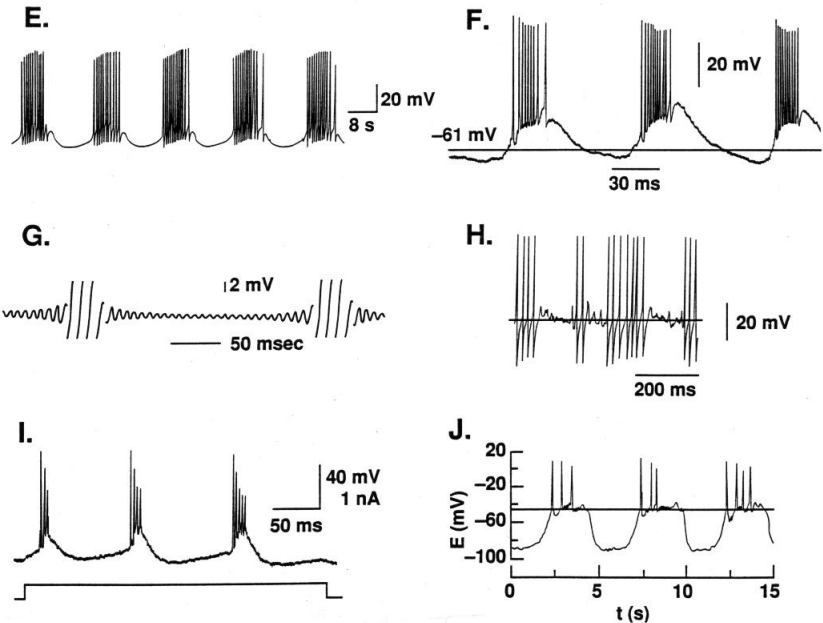
\includegraphics[width=\textwidth]{bursting_examples}
\end{figure}

\end{columns}
\end{frame}

\begin{frame}
\frametitle{Bursting}
\framesubtitle{Three variables and three time-scales}
\begin{itemize}
\item Like FitzHugh-Nagumo, but with third (ultra-slow) state
\item Ultra slow process modulates the fast processes
\end{itemize}

\begin{figure}
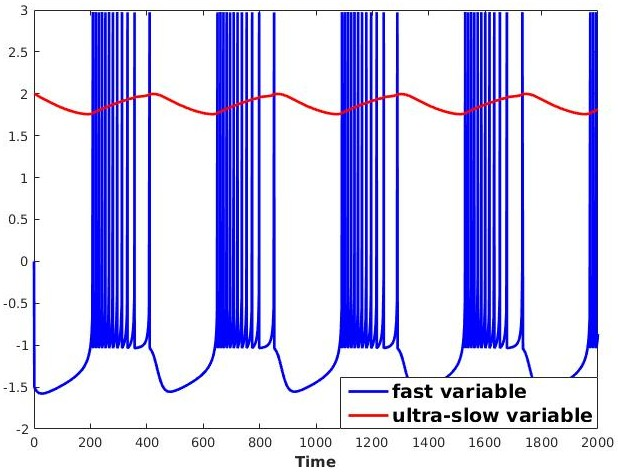
\includegraphics[width=0.7\textwidth]{hRose_bursting2}
\end{figure}

\end{frame}

\begin{frame}
\frametitle{A bursting normal form}
\framesubtitle{Franci and Sepulchre. \emph{Realization of nonlinear behaviours from organizing centers.} (2014)\newline
Drion et al. \emph{Neuoronal behaviors: a control perspective.} (2015)}
\begin{columns}
\column{0.6\textwidth}
\begin{figure}
\includegraphics<1>[width=\textwidth]{tts_circuit}
\includegraphics<2>[width=\textwidth]{tts_circuit1}
\includegraphics<3>[width=\textwidth]{tts_circuit2}
\includegraphics<4>[width=\textwidth]{tts_circuit}
\end{figure}
\column{0.4\textwidth}
\begin{figure}
\includegraphics<1>[width=\textwidth]{feedback_interactions2}
\includegraphics<2>[width=\textwidth]{feedback_interactions3}
\includegraphics<3>[width=\textwidth]{feedback_interactions4}
\includegraphics<4>[width=\textwidth]{feedback_interactions2}
\end{figure}
\end{columns}
\end{frame}

\begin{frame}
\frametitle{Bursting and Relay feedback}
\centering
\tikzstyle{block} = [draw,  rectangle,  minimum height=3em, minimum width=6em]
\tikzstyle{gain} = [draw, regular polygon, regular polygon sides = 3, regular polygon rotate = 90, minimum height = 2em, minimum width = 2em]
\tikzstyle{gain2} = [draw, regular polygon, regular polygon sides = 3, regular polygon rotate = 30, minimum height = 2em, minimum width = 2em]
\tikzstyle{sum} = [draw,  circle, node distance=1cm]
%\tikzstyle{input} = [coordinate]
%\tikzstyle{output} = [coordinate]
\tikzstyle{pinstyle} = [pin edge={to-,thin,black}]

\def\relayA
{
	\tikz[remember picture,overlay]
	{
		\draw[->] (-.8,0) -- (.8,0);
		\draw[->] (0,-0.45)--(0,0.45);
		\draw[blue] (-0.7,-0.2)--(0.2,-0.2)--(0.2,0.2)--(.7,.2);
		\draw[blue] (.2,.2)--(-.2,.2)--(-.2,-.2);
		\node at (-.35,0.1) {\tiny$\epsilon_2$};
		\node at (.35,-.1) {\tiny$\epsilon_1$};
				\node at (0.6, 0.3) {\tiny$1$};
		\node at (-0.6,-0.3){\tiny$-1$};
	}
}

\def\relayB
{
	\tikz[remember picture,overlay]
	{
		\draw[->] (-.8,0) -- (.8,0);
		\draw[->] (0,-0.45)--(0,0.45);
		\draw[blue] (-0.7,-0.2)--(0.2,-0.2)--(0.2,0.2)--(.7,.2);
		\draw[blue] (.2,.2)--(-.2,.2)--(-.2,-.2);
		\node at (-.55,0.1) {\tiny$\alpha_{min}$};
		\node at (.55,-.15) {\tiny$\alpha_{max}$};
		\node at (0.6, 0.3) {\tiny$\langle x_f \rangle$};
		\node at (-0.6,-0.3){\tiny$-1$};
	}
}

\resizebox{10cm}{!}{%
  % The block diagram code is probably more verbose than necessary
  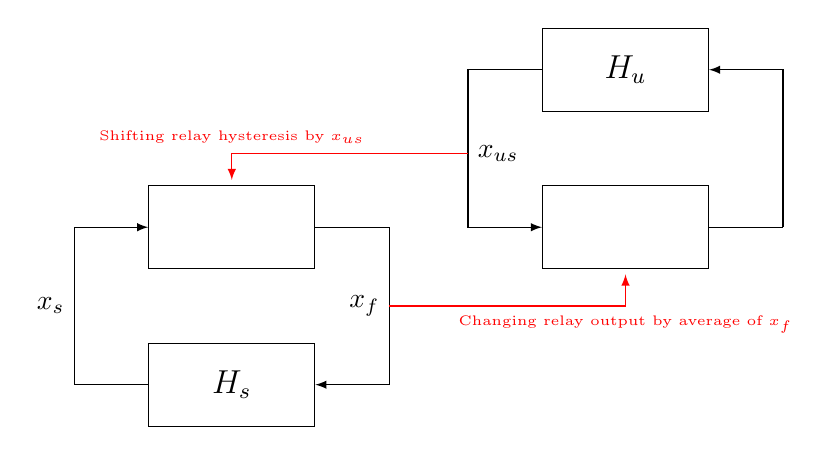
\begin{tikzpicture}[auto, node distance=2cm,>=latex,scale=1]
      % We start by placing the blocks
      % Fast slow system
      \node at (-3,-1) (input1){};
      \node [block, right of = input1](relay1){};
      \node [] at (relay1) {\relayA};
      \node [coordinate, above of = relay1, node distance = 0.6cm](relay1_top){};
      \node [coordinate, right of = relay1] (endA) {};
      \node [block, below of = relay1] (Hs) {\large $H_s$};
      
      % Ultra slow system
      \node [block, right of = endA, node distance = 3cm](relay2){};
      \node [] at (relay2) {\relayB};
      \node [coordinate, below of = relay2, node distance = 0.6cm](relay2_top){};
      \node [coordinate, right of = relay2](endB){};
      \node [block, above of = relay2](Hus){\large $H_{u}$};
      \node [left of = Hus](inB){};

      % Once the nodes are placed, connecting them is easy. %

     % fast-slow loop
     \draw[->](-3,-1)--(relay1);
     \draw[-](relay1)--(endA);
     \draw[->](endA)|- node[name = xf,near start,left]{$x_f$} (Hs);
     \draw[-](Hs)-| node[name = xs,near end]{$x_s$}(-3,-1);

	% ultra-slow loop
	\draw[-](relay2)--(endB);
	\draw[->](endB)|-(Hus); 
	\draw[-](Hus)--(inB);
	\draw[->](inB)|- node[name = alpha, near start]{$x_{us}$}(relay2);
	\draw[-](Hus)-|(2,0);
     
     % coupling
     \draw[->,red](xf)-|node[below]{\tiny{Changing relay output by average of $x_f$}}(relay2_top);
     \draw[->,red](alpha)-|node[above]{\tiny{Shifting relay hysteresis by $x_{us}$}}(relay1_top);

  \end{tikzpicture}
}
\end{frame}




\section{Conclusions}

\subsection{Conclusion}
\begin{frame}
\frametitle{Conclusions}
	\begin{itemize}
	\item Modelled simple oscillations using relay feedback
	\begin{itemize}
	\item Goodwin oscillator model
	\item FitzHugh-Nagumo model
	\end{itemize}
	\item Modelled a complex oscillation using relay feedback
	\begin{itemize}
	\item Bursting normal form model
	\item Hindmarsh-Rose model
	\end{itemize}
	\item Appealing framework
	\begin{itemize}
	\item Tractable in high dimensions $\rightarrow$ excitable systems
	\item Predict stability, time periods,  initial conditions
	\end{itemize}
	\end{itemize}
\end{frame}

\end{document}
